\documentclass[aspectratio=169]{beamer}
\usepackage{pgf}
\usepackage{colortbl,tabularx,mathrsfs,calligra,xcolor}
\usepackage{amsmath,amsfonts,amssymb,amsthm}
    \DeclareMathOperator{\sign}{sgn}
\usepackage{ragged2e}
\usepackage{setspace}
\usepackage{filecontents}
\usepackage{caption}
\usepackage{subcaption}
\usepackage{contour}
\usepackage{fancybox}
\usepackage{wrapfig}
\usepackage{multirow}
\usepackage{multicol}
\usepackage{tikz, pgfplots, tkz-euclide,calc}
    \usetikzlibrary{patterns,snakes,shapes.arrows,shapes.geometric,fit}
\usepackage{listings}
\usepackage{pifont}
\usepackage[scaled]{uarial}
\renewcommand*\familydefault{\sfdefault} %% Only if the base font of the document is to be sans serif
\usepackage[T1]{fontenc}

\graphicspath{{C:/Users/teoso/OneDrive/Documents/Asisten Dosen & Lab/Asisten Dosen/PPT Kalkulus/Gambar & Logo/}{D:/Hada Touya/Asisten-things/Asisten Dosen/PPT Kalkulus/Gambar & Logo/}}

\definecolor{HIMAmuda}{HTML}{01D1FD}
\definecolor{HIMAtua}{HTML}{02016A}
\definecolor{HIMAabu}{HTML}{CBCBCC}
\definecolor{PastelGreen}{HTML}{77DD77}

\usetheme{Madrid}

\setbeamercolor{palette primary}{bg=HIMAtua,fg=white}
\setbeamercolor{palette secondary}{bg=HIMAmuda,fg=black}
\setbeamercolor{palette tertiary}{bg=HIMAabu,fg=black}
\setbeamercolor{palette quaternary}{bg=HIMAmuda,fg=white}
\setbeamercolor{structure}{fg=HIMAmuda} % itemize, enumerate, etc
\setbeamercolor{section in toc}{fg=HIMAtua} % TOC sections
\setbeamercolor{block title alerted}{fg=white,bg=magenta}
\setbeamercolor{block body alerted}{fg=black!90,bg=pink}

\usefonttheme{professionalfonts}
\setbeamertemplate{theorems}[numbered]

\usebackgroundtemplate{%
\tikz[overlay,remember picture] \node[opacity=0.1, at=(current page.center)]{
\includegraphics[width=\paperwidth]{arona class}};
}

\renewcommand\thesubfigure{\arabic{subfigure}}
\newtheorem*{funfact}{Fun Fact}
\newtheorem{latihan}{Latihan}
\newtheorem{definisi}{Definisi}
\newtheorem{teorema}{Teorema}
\theoremstyle{definition}
\newtheorem*{contoh}{Contoh}
\newcommand{\R}{\mathbb{R}}

\AtBeginEnvironment{funfact}{%
  \setbeamercolor{block title}{fg=white,bg=PastelGreen} % Set title background to pastel green and text to white
  \setbeamercolor{block body}{parent=normal text,bg=PastelGreen!30!white} % Set body background to a lighter pastel green
}
\AtBeginEnvironment{definisi}{
    \setbeamercolor{block title}{fg=white,bg=HIMAtua}
    \setbeamercolor{block body}{parent=normal text,bg=HIMAtua!30!white}
    \setbeamercolor{item}{fg=HIMAtua}
}
\AtBeginEnvironment{teorema}{
    \setbeamercolor{block title}{bg=darkgray,fg=white}
    \setbeamercolor{block body}{parent=pallette tertiary,bg=HIMAabu!30!white}
}
\AtBeginEnvironment{contoh}{%
  \setbeamercolor{block title}{fg=white,bg=PastelGreen} % Set title background to pastel green and text to white
  \setbeamercolor{block body}{parent=normal text,bg=PastelGreen!30!white} 
}
\AtBeginEnvironment{alertblock}{%
  \setbeamercolor{item}{fg=red}
}



\author[Tetew]{Teosofi Hidayah Agung}
\date{19 September 2024}
\title[Kalkulus 1 - Bab 3]{Limit dan Kekontinuan}
\institute[Matematika ITS]{Departemen Matematika\\ Institut Teknologi Sepuluh Nopember}
\titlegraphic{{
\includegraphics[scale=0.3]{ITS.png}$\quad$
\includegraphics[scale=0.02]{M.png}}}

\newcommand{\dom}{\mathcal{D}}
\newcommand{\rng}{\mathcal{R}}

\renewcommand{\arraystretch}{1.5}

\begin{document}
{\usebackgroundtemplate{
    \tikz[overlay,remember picture] \node[opacity=0.09, at=(current page.center)]{
\includegraphics[width=\paperwidth]{limitless}};}
\begin{frame}
    \titlepage
\end{frame}
}

\begin{frame}{Daftar isi}
    \tableofcontents[currentsection]
\end{frame}

\section{Notasi Limit}
\begin{frame}
    \frametitle{\insertsection}
    \begin{definisi}
        Notasi limit yang biasanya dibaca ``limit $f(x)$ saat $x$ \textbf{mendekati} $a$ adalah $L$'' dituliskan sebagai
        \[\lim_{x\to a} f(x)=L,\]
        Artinya jika kita mengambil nilai $x$ yang sangat dekat dengan $a$, maka $f(x)$ akan sangat dekat dengan $L$.
    \end{definisi}
    \onslide<2->{
        \setbeamercolor{item}{fg=PastelGreen!50!HIMAmuda}
        \begin{alertblock}{Catatan}
            \begin{itemize}
                \item Kata ``mendekati'' jangan disamakan dengan ``menuju''.
                \item Nilai $f(a)$ tidak harus sama dengan $L$ atau bahkan $f(a)$ tidak terdefinisi.
                \item Nilai $f(x)$ untuk $x=a$ tidak mempengaruhi nilai limit.
            \end{itemize}
        \end{alertblock}}
\end{frame}

\begin{frame}
    \frametitle{\insertsection}
    \begin{block}{Fungsi Piecewise}
        Fungsi piecewise(sepotong-sepotong) adalah fungsi yang didefinisikan dengan beberapa aturan berbeda pada interval yang berbeda. Secara umum dapat ditulis sebagai berikut
        \begin{equation*}
            f(x)=\begin{cases}
                f_1(x), & x\in \dom_1 \\
                f_2(x), & x\in \dom_2 \\
                        & \vdots      \\
                f_n(x), & x\in \dom_n
            \end{cases}
        \end{equation*}
        dengan $\dom_1\cup\dom_2\cup\cdots\cup\dom_n=\dom_f$ dan $\dom_i\cap\dom_j=\emptyset$ untuk $i\neq j$
    \end{block}
\end{frame}

\begin{frame}
    \frametitle{\insertsection}
    \begin{contoh}
        \begin{itemize}
            \item $f(x)=|x|$
            \item $f(x)=\sign(x)=\begin{cases}
                          1,  & x>0 \\
                          0,  & x=0 \\
                          -1, & x<0
                      \end{cases}$
            \item $f(x)=\begin{cases}
                          x+2,      & x\geq 2 \\
                          -x^2-x+6, & x<2
                      \end{cases}$
        \end{itemize}
    \end{contoh}
\end{frame}

\section{Perhitungan Limit}
\begin{frame}
    \frametitle{\insertsection}
    \begin{definisi}
        Domain fungsi $f$ adalah himpunan semua nilai $x$ yang memenuhi $f(x)$ didefinisikan. Notasi domain fungsi $f$ adalah \[\dom(f)=\{x\in\R\mid f(x)\text{ terdefinisi}\}\]
        Range fungsi $f$ adalah himpunan semua nilai $f(x)$ yang mungkin diperoleh saat $x$ berjalan di domain fungsi $f$. Notasi range fungsi $f$ adalah \[\rng(f)=\{f(x)\mid x\in\dom(f)\}\]
    \end{definisi}
\end{frame}

\begin{frame}
    \frametitle{\insertsection}
    \begin{table}
        \centering
        \begin{tabular}{|c|c|c|c|c|}
            \hline
            \rowcolor{HIMAmuda}
                                                & \multicolumn{2}{c|}{\textbf{Domain}} & \multicolumn{2}{c|}{\textbf{Range}}                                                           \\
            \cline{2-5}
            \rowcolor{HIMAmuda}
            \multirow{-2}{*}{\textbf{Fungsi}}   & \textbf{Himpunan}                    & \textbf{Interval}                   & \textbf{Himpunan}         & \textbf{Interval}           \\
            \hline
            $f(x)=ax+b$                         & $\R$                                 & $(-\infty,\infty)$                  & $\R$                      & $(-\infty,\infty)$          \\
            $f(x)=a(x-p)^2+q$                   & $\R$                                 & $(-\infty,\infty)$                  & $\{f(x)\mid f(x)\geq q\}$ & $[q,\infty)$                \\
            $\displaystyle f(x)=\frac{1}{g(x)}$ & $\{x\mid g(x)\ne 0\}$                & $(-\infty,\infty)$                  & $\{f(x)\mid f(x)\ne 0\}$  & $(-\infty,0)\cup(0,\infty)$ \\
            $f(x)=\sqrt{g(x)}$                  & $\{x\mid g(x)\geq 0\}$               & $[0,\infty)$                        & $\{f(x)\mid f(x)\geq 0\}$ & $[0,\infty)$                \\
            \hline
        \end{tabular}
        \caption{Domain dan Range beberapa fungsi}
    \end{table}
\end{frame}

\begin{frame}
    \frametitle{\insertsection}
    \begin{exampleblock}{Latihan}
        \begin{enumerate}
            \item Jika $f(t)=\begin{cases}
                          2t+1,  & t\geq 0 \\
                          t^2-1, & t<0
                      \end{cases}$, tentukan $f(x^2)$
            \item Tulislah dalam fungsi sepotong-sepotong $f(x)=|4+|x-1||$
            \item Tentukan domain dan range dari fungsi $\displaystyle f(x)=\frac{1}{\sqrt{4-x^2}}$
        \end{enumerate}
    \end{exampleblock}
\end{frame}

\section{Limit di Tak-Hingga}
\begin{frame}
    \frametitle{\insertsection}
    \begin{definisi}
        Misalkan $f$ dan $g$ adalah dua fungsi. Operasi-operasi pada fungsi adalah sebagai berikut
        \begin{enumerate}
            \item Penjumlahan: $(f+g)(x)=f(x)+g(x)$
            \item Pengurangan: $(f-g)(x)=f(x)-g(x)$
            \item Perkalian: $(f\cdot g)(x)=f(x)\cdot g(x)$
            \item Pembagian: $\left(\displaystyle\frac{f}{g}\right)(x)=\displaystyle\frac{f(x)}{g(x)}$
        \end{enumerate}
        Kemudian untuk domain dari fungsi hasil operasi adalah \[\dom(f\pm g)=\dom(f\cdot g)=\dom(f)\cap\dom(g)\]
        Sedangkan untuk kasus pembagian harus memenuhi $g(x)\ne 0$, sehingga
        \[\dom\left(f/g\right)=(\dom(f)\cap\dom(g)) - \{x\mid g(x)=0\}\]
    \end{definisi}
\end{frame}

\begin{frame}
    \frametitle{\insertsection}
    \begin{definisi}
        Komposisi fungsi $f$ dan $g$ adalah fungsi baru yang didefinisikan sebagai
        \[(f\circ g)(x)=f(g(x))\]
        Domain dari fungsi komposisi adalah
        \[\dom(f\circ g)=\{x\in\dom(g)\mid g(x)\in\dom(f)\}\]
    \end{definisi}
\end{frame}

\begin{frame}
    \frametitle{\insertsection}
    \begin{exampleblock}{Latihan}
        \begin{enumerate}
            \item Domain dari fungsi $\displaystyle f(x)=\frac{1}{x}+\sqrt{4-x^2}$ adalah
            \item Jika $f(g(x))=x^2+1$ dan $f(x)=\sqrt{x-1}$, tentukan $g(x)$
            \item Tentukan domain dari $g\circ f$ jika $f(x)=\sqrt{x^2-9}$ dan $\displaystyle g(x)=\frac{2}{x-3}$
        \end{enumerate}
    \end{exampleblock}
\end{frame}

\section{Kekontinuan}
\begin{frame}
    \frametitle{\insertsection}
    \begin{definisi}
        Grafik fungsi $f$ adalah himpunan semua titik $(x,y)$ dalam koordinat kartesius yang memenuhi persamaan $y=f(x)$.
    \end{definisi}
    \onslide<2->{\begin{teorema}
            Misalkan $y=f(x)$ adalah fungsi real, maka grafik $f(-x)$ adalah refleksi terhadap sumbu $y$ dari grafik $f(x)$ dan grafik $-f(x)$ adalah refleksi terhadap sumbu $x$ dari grafik $f(x)$.
        \end{teorema}}
\end{frame}

\begin{frame}
    \frametitle{\insertsection}
    Kasus $f(x)\implies f(-x)$
    \begin{figure}
        \begin{minipage}[b]{0.45\textwidth}
            \centering
            \begin{tikzpicture}[scale=0.8]
                \draw [->] (-2,0) -- (3,0) node [right] {\footnotesize$x$};
                \draw [->] (0,-1) -- (0,3) node [above] {\footnotesize$y$};

                \draw [domain=-1:3, samples=50, thick, blue] plot (\x, {sqrt(\x+1)});
                \node [below] at (-1,0) {\footnotesize$-1$};
            \end{tikzpicture}
            \caption*{$\boxed{y=\sqrt{x+1}}$}
        \end{minipage}
        \onslide<2->{\begin{minipage}[b]{0.45\textwidth}
                \centering
                \begin{tikzpicture}[scale=0.8]
                    \draw [->] (-3,0) -- (2,0) node [right] {\footnotesize$x$};
                    \draw [->] (0,-1) -- (0,3) node [above] {\footnotesize$y$};

                    \draw [domain=-1:2, samples=50, thick, cyan, dashed] plot (\x, {sqrt(\x+1)});
                    \draw [domain=-3:1, samples=50, thick, blue] plot (\x, {sqrt(-\x+1)});
                    \node [below] at (-1,0) {\footnotesize$-1$};
                    \node [below] at (1,0) {\footnotesize$1$};
                \end{tikzpicture}
                \caption*{$\boxed{y=\sqrt{-x+1}}$}
            \end{minipage}}
    \end{figure}
\end{frame}

\begin{frame}
    \frametitle{\insertsection}
    Kasus $f(x)\implies -f(x)$
    \begin{figure}
        \begin{minipage}[b]{0.45\textwidth}
            \centering
            \begin{tikzpicture}[scale=0.8]
                \draw [->] (-2,0) -- (4,0) node [right] {\footnotesize$x$};
                \draw [->] (0,-3) -- (0,3) node [above] {\footnotesize$y$};

                \draw [domain=1.35:4, samples=50, thick, blue] plot (\x, {1/(\x-1)});
                \draw [domain=-2:0.65, samples=50, thick, blue] plot (\x, {1/(\x-1)});
                \draw [domain=-3:3, samples=10, darkgray, dashed] plot (1, {\x});

                \node [below right] at (1,0) {\footnotesize$1$};
            \end{tikzpicture}
            \caption*{$\boxed{y=\frac{1}{x-1}}$}
        \end{minipage}
        \onslide<2->{\begin{minipage}[b]{0.45\textwidth}
                \centering
                \begin{tikzpicture}[scale=0.8]
                    \draw [->] (-2,0) -- (4,0) node [right] {\footnotesize$x$};
                    \draw [->] (0,-3) -- (0,3) node [above] {\footnotesize$y$};

                    \draw [domain=1.35:4, samples=50, thick, cyan, dashed] plot (\x, {1/(\x-1)});
                    \draw [domain=-2:0.65, samples=50, thick, cyan, dashed] plot (\x, {1/(\x-1)});
                    \draw [domain=-3:3, samples=10, darkgray, dashed] plot (1, {\x});

                    \draw [domain=1.35:4, samples=50, thick, blue] plot (\x, {1/(1-\x)});
                    \draw [domain=-2:0.65, samples=50, thick, blue] plot (\x, {1/(1-\x)});

                    \node [below right] at (1,0) {\footnotesize$1$};
                \end{tikzpicture}
                \caption*{$\boxed{y=\frac{1}{1-x}}$}
            \end{minipage}}
    \end{figure}
\end{frame}

\begin{frame}
    \frametitle{\insertsection}
    Gambarkan grafik fungsi $y=f(x)=\begin{cases}
            -x^2+4, & x\geq 1 \\
            x+1,    & x<1
        \end{cases}$
    \begin{figure}
        \begin{minipage}[b]{0.45\textwidth}
            \centering
            \begin{tikzpicture}[scale=0.8]
                \draw [->] (-3,0) -- (3,0) node [right] {\footnotesize$x$};
                \draw [->] (0,-1) -- (0,5) node [above] {\footnotesize$y$};

                \draw [domain=-2.2:2.2, samples=50, thick, blue] plot (\x, {-(\x)^2+4});
                \node [below] at (2,0) {\footnotesize$2$};
                \node [below] at (-2,0) {\footnotesize$-2$};
            \end{tikzpicture}
            \caption*{$\boxed{y=-x^2+4}$}
        \end{minipage}
        \begin{minipage}[b]{0.45\textwidth}
            \centering
            \begin{tikzpicture}[scale=0.8]
                \draw [->] (-4,0) -- (2,0) node [right] {\footnotesize$x$};
                \draw [->] (0,-3) -- (0,3) node [above] {\footnotesize$y$};

                \draw [domain=-3.5:1.5, samples=50, thick, blue] plot (\x, {\x+1});
                \node [below] at (-1,0) {\footnotesize$-1$};
            \end{tikzpicture}
            \caption*{$\boxed{y=x+1}$}
        \end{minipage}
    \end{figure}
\end{frame}

\begin{frame}
    \frametitle{\insertsection}
    \begin{figure}
        \begin{minipage}[b]{0.45\textwidth}
            \centering
            \begin{tikzpicture}[scale=0.8]
                \draw [->] (-3,0) -- (3,0) node [right] {\footnotesize$x$};
                \draw [->] (0,-1) -- (0,5) node [above] {\footnotesize$y$};

                \draw [domain=1:2.2, samples=50, thick, blue] plot (\x, {-(\x)^2+4});
                \draw [domain=-2.2:1, samples=50, thick, cyan, dashed] plot (\x, {-(\x)^2+4});

                \draw [domain=-1:5, samples=10, darkgray, dashed] plot (1, {\x});
                \draw[fill=blue] (1,3) circle (0.1);

                \node [below] at (2,0) {\footnotesize$2$};
                \node [below] at (-2,0) {\footnotesize$-2$};
                \node [below right] at (1,0) {\footnotesize$1$};
            \end{tikzpicture}
            \caption*{$\boxed{y=-x^2+4,\,x\geq 1}$}
        \end{minipage}
        \begin{minipage}[b]{0.45\textwidth}
            \centering
            \begin{tikzpicture}[scale=0.8]
                \draw [->] (-4,0) -- (2,0) node [right] {\footnotesize$x$};
                \draw [->] (0,-3) -- (0,3) node [above] {\footnotesize$y$};

                \draw [domain=1:1.5, samples=50, thick, cyan, dashed] plot (\x, {\x+1});
                \draw [domain=-3.5:1, samples=50, thick, blue] plot (\x, {\x+1});

                \draw [domain=-3:3, samples=10, darkgray, dashed] plot (1, {\x});
                \draw[fill=white] (1,2) circle (0.1);

                \node [below] at (-1,0) {\footnotesize$-1$};
                \node [below right] at (1,0) {\footnotesize$1$};
            \end{tikzpicture}
            \caption*{$\boxed{y=x+1,\,x<1}$}
        \end{minipage}
    \end{figure}
\end{frame}

\begin{frame}
    \frametitle{\insertsection}
    Jadi, grafik fungsi $y=f(x)=\begin{cases}
            -x^2+4, & x\geq 1 \\
            x+1,    & x<1
        \end{cases}$ adalah
    \begin{figure}
        \centering
        \begin{tikzpicture}[scale=0.8]
            \draw [->] (-3,0) -- (3,0) node [right] {\footnotesize$x$};
            \draw [->] (0,-2) -- (0,4) node [above] {\footnotesize$y$};

            \draw [domain=1:2.2, samples=50, thick, blue] plot (\x, {-(\x)^2+4});
            \draw [domain=-2:1, samples=50, thick, blue] plot (\x, {\x+1});

            \draw [domain=2:3, samples=10, darkgray, dashed] plot (1, {\x});
            \draw[fill=blue] (1,3) circle (0.1);
            \draw[fill=white] (1,2) circle (0.1);

            \node [below] at (2,0) {\footnotesize$2$};
            \node [below] at (-1,0) {\footnotesize$-1$};
            \node [below] at (1,0) {\footnotesize$1$};
        \end{tikzpicture}
    \end{figure}
\end{frame}

\begin{frame}
    \frametitle{\insertsection}
    \begin{exampleblock}{Latihan}
        \begin{enumerate}
            \item Tentukan persamaan dari grafik fungsi berikut\\
                  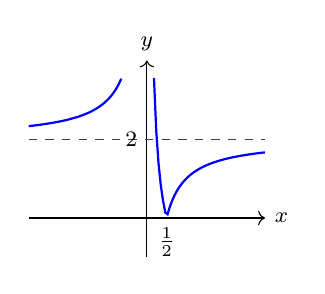
\begin{tikzpicture}[scale=0.5]
                      \draw [->] (-3,0) -- (3,0) node [right] {\footnotesize$x$};
                      \draw [->] (0,-1) -- (0,4) node [above] {\footnotesize$y$};

                      \draw [domain=-3:-0.65, samples=50, thick, blue] plot (\x, {abs((1/\x)-2)});
                      \draw [domain=0.18:3, samples=50, thick, blue] plot (\x, {abs((1/\x)-2)});

                      \draw [domain=-3:3, samples=10, darkgray, dashed] plot ({\x},2);

                      \node [left] at (0,2) {\footnotesize$2$};
                      \node [below] at (0.5,0) {\footnotesize$\frac{1}{2}$};
                  \end{tikzpicture}
            \item Gambarkan fungsi $f(x)=|4+|x-1||$
        \end{enumerate}
    \end{exampleblock}
\end{frame}

\end{document}